In the last section we have seen that $\QC_{m,n}\subsetneq \LC_{m,n}$. In this section we will prove the fact that $\QC_{m,n}\subset K\LC_{m,n}$ for some universal constant $K$ independent of $m$ and $n$. In particular, we can show that the smallest constant $K$ so that the above inclusion holds true the Grothendieck constant $K_G\leq \pi/2\ln(1+\sqrt{2})$ is. 

\subsection{Grothendieck's Inequality}
	\begin{lemma}[Grothendieck's identity]\label{lem:G_id}
		Let $x,y\in\mathbb{R}^d$ be unit vectors. Let $r\in\mathbb{R}^d$ be a random unit vector chosen from $O(d)$-invariant probability distribution on the unit sphere. Then
		\begin{enumerate}
			\item[i,] $\mathbb{P}[\sgn(\sclr{x}{r})\neq\sgn(\sclr{y}{r})]=\frac{\arccos(\sclr{x}{y})}{\pi}$
			\item[ii,] $\mathbb{E}[\sgn(\sclr{x}{r})\sgn(\sclr{y}{r})]=\frac{2}{\pi}\arcsin(\sclr{x}{y}).$
		\end{enumerate}
	\end{lemma}
	\begin{proof}
		For the proof of $i,$ assume that $x$ and $y$ are linearly dependent. Since both, $x$ and $y$, are unit vectors, $\arccos(\sclr{x}{y}) = \arccos(1)=0$ if $x=y$ or $\arccos(\sclr{x}{y}) = \arccos(-1) = \pi$ if $x=-y$.
		
		Conversely assume that $x$ and $y$ are linearly independent, i.\,e. $\operatorname{dim}(\spn\{x,y\})=2$. Now project $r$ orthogonally on the plane spanned by $x$ and $y$. This gives us a vector $s\in \spn\{x,y\}$ with $\sclr{x}{r} = \sclr{x}{s}$ and $\sclr{y}{r} = \sclr{y}{s}$. The unit vector $n\coloneqq s/\modul{s}$ is uniformly distributed on the \textcolor{red}{unit circle/disk} that occurs if we consider the intersection of the unit sphere and $\spn\{x,y\}$ by the $O(d)$-invariance of the probability distribution. \\
		
		\noindent\begin{minipage}{\textwidth}	
			If $n$ lies on the segment of the unit circle induced by the green part, the angle between $x$ and $n$ as well as between $y$ and $n$ is smaller than $\pi/2$, hence $\sclr{x}{n}$ and $\sclr{y}{n}$ are positive. 
			\begin{wrapfigure}{r}{0.4\textwidth}
				\vspace{-20pt}
				\begin{center}
					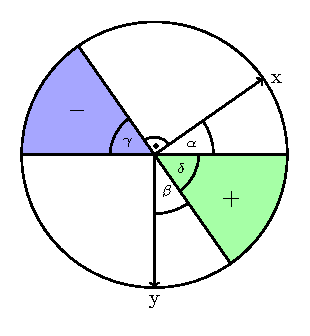
\includegraphics[width=0.38\textwidth]{chapters/fig_unit_circle.pdf}
				\end{center}
				\vspace{-20pt}
			\end{wrapfigure}
			Otherwise, if $n$ lies on the segment of the unit circle induced by the blue part, the angle between both $x$ and $n$ as well as $y$ and $n$ is greater than $3\pi/2$, hence $\sclr{x}{n}$ and $\sclr{y}{n}$ are negative.
			
			\hspace{12pt} Now, if we want to calculate the probability that the signs of the two scalar products disagree, we are interested in the undyed segments of the unit circle. Thus, it is sufficient to calculate the periphery of the undyed segments of the circle. In particular on the unit circle, the angle between two vectors equals the periphery of the segment of the circle between those two vectors. 
				
			\hspace{12pt} Because $\gamma$ and $\delta$ are vertical angles they are both equal. Furthermore, $\alpha$ and $\beta$ have to be equal too, since $\gamma$ and $\delta$ are equal and $\alpha+\delta = \beta+\gamma = \pi/2$. With $\alpha = \arccos(\sclr{x}{y}) - \pi/2$ the first part of Lemma \ref{lem:G_id} follows:
		\end{minipage}
		\begin{align*}
			\mathbb{P}[\sgn(\sclr{x}{n})\neq\sgn(\sclr{y}{n})]=2\frac{\frac{\pi}{2}+\alpha}{2\pi} = \frac{\arccos(\sclr{x}{y})}{\pi}.
		\end{align*}
		
		\noindent We conclude with the proof of the second part of Lemma \ref{lem:G_id}: 
		\begin{align*}
			&\mathbb{E}[\sgn(\sclr{x}{r}) \sgn(\sclr{y}{r})] \\
			&\qquad= 1\cdot\mathbb{P}[\sgn(\sclr{x}{r}) = \sgn (\sclr{y}{r} )] - 1\cdot \mathbb{P}[\sgn(\sclr{x}{r}) \neq \sgn(\sclr{y}{r})] \\
			&\qquad= 1 - 2\mathbb{P}[\sgn(\sclr{x}{r}) \neq \sgn(\sclr{y}{r})] \\
			&\qquad= 1 - 2 \frac{\arccos(\sclr{x}{y})}{\pi} \\
			&\qquad= \frac{2}{\pi} \arcsin(\sclr{x}{y}),
		\end{align*}
		because $\arcsin (t) + \arccos(t) = \pi/2$.
	\end{proof}
	
	\begin{lemma}[Krivine's trick]\label{lem:krivines_trick}
		Let $x_1,\dots,x_m,y_1,\dots,y_n\in S^{m+n-1}$ be given. Furthermore, let $r\in S^{n+m-1}$ be a random unit vector chosen form the $O(n+m-1)$-invariant probability distribution on the unit sphere. Then there are $x_1^\prime,\dots,x_m^\prime, y_1^\prime,\dots,y_n^\prime\in S^{m+n-1}$ so that
		\begin{equation}
			\mathbb{E}[\sgn(\sclr{x_i^\prime}{r})\sgn(\sclr{y_j^\prime}{r})] = \beta \sclr{x_i}{y_j},
			\label{eq:krivines_trick}
		\end{equation}		
		with $\beta = \frac{2}{\pi} \ln (1+\sqrt{2}).$
	\end{lemma}
	
	\noindent For the proof of \ref{lem:krivines_trick} we need to use the $k$-th tensor product of $\mathbb{R}^n$. The $\mathbb{R}^n$ is an $n$-dimensional Euclidean space with inner product \sclr{\cdot}{\cdot} and orthonormal basis $e_1,\dots,e_n$. The \emph{$k$-th tensor product of $\mathbb{R}^n$} is denoted by $(\mathbb{R}^n)^{\tensor k}$ and it is a Euclidean  vector space of dimension $n^k$ with orthonormal basis $e_{i_1}\tensor e_{i_2} \tensor \cdots \tensor e_{i_k}$, $i_l\in\{1,\dots,n\}$. In particular
	\begin{align}
		\sclr{e_{i_1}\tensor \cdots \tensor e_{i_k}}{e_{j_1}\tensor \cdots \tensor e_{j_k}}
		&= \prod_{l=1}^k \sclr{e_{i_l}}{e_{j_l}}\nonumber\\
		&=\begin{cases}
			1 & , \text{ if } i_l=j_l \text{ for all } l=1,\dots,n,\\
			0 & , \text{ otherwise},
		\end{cases} \label{eq:orthonormtensor}
	\end{align}
	and for $v\in\mathbb{R}^n$ with $v=v_1e_1+\cdots +v_ne_n$ we define $v^{\tensor k} \in (\mathbb{R}^n)^{\tensor k}$ by 
	\begin{equation}
		v^{\tensor k} \coloneqq (v_1e_1 + \cdots + v_ne_n) \tensor \cdots \tensor (v_1e_1 + \cdots + v_ne_n) = \sum_{i_1,\dots,i_k} v_{i_1}\cdots v_{i_k} e_{i_1}\tensor\cdots\tensor e_{i_k},
	\end{equation}
	where the last equation follows by the distributive law (identity $ii,$ of the tensor product). 
	Thus, for $v,w\in\mathbb{R}^n$ 
	\begin{align}
		\sclr{v^{\tensor k}}{w^{\tensor k}}
	%	&\overset{\textcolor{white}{\eqref*{eq:orthonormtensor}}}{=} \sum_{i_1,\dots,i_k} v_{i_1}\cdots v_{i_k}\left(e_{i_1}\tensor\cdots\tensor e_{i_k}\right)^\top \sum_{j_1,\dots,j_k} w_{j_1}\cdots w_{j_k}(e_{j_1}\tensor\cdots\tensor e_{j_k}) \nonumber\\
		&\overset{\textcolor{white}{\eqref*{eq:orthonormtensor}}}{=} \sum_{i_1,\dots,i_k} v_{i_1}\cdots v_{i_k} \sum_{j_1,\dots,j_k} w_{j_1}\cdots w_{j_k} \sclr{e_{i_1}\tensor\cdots\tensor e_{i_k}}{e_{j_1}\tensor\cdots\tensor e_{j_k}} \nonumber\\
		&\overset{\eqref{eq:orthonormtensor}}{=} \sum_{i_1,\dots,i_k} v_{i_1}\cdots v_{i_k}w_{i_1}\cdots w_{i_k} \nonumber\\
		&\overset{\textcolor{white}{\eqref*{eq:orthonormtensor}}}{=}(\sum_{i=1}^n v_iw_i)^k = \sclr{v}{w}^k. \label{eq:kth_tensor}
	\end{align}
	\begin{proof}
		Define the function $E: [-1,+1] \to [-1,+1]$ by $E(t)=\frac{2}{\pi}\arcsin(t)$. Due to Grothendieck's identity (Lemma \ref{lem:G_id}):
		\begin{align*}
			E(\sclr{x_i^\prime}{y_j^\prime} ) &= \mathbb{E}[\sgn(\sclr{x_i^\prime}{r})\sgn(\sclr{y_j^\prime}{r})]\\
			&\overset{!}{=}\beta \sclr{x_i}{y_j}.
		\end{align*}
		
		\noindent Idea: To find $\beta,x_i^\prime,y_j^\prime$ we invert $E$:
		\[
			\sclr{x_i^\prime}{y_j^\prime} = E^{-1} (\beta \sclr{x_i}{y_j})	
		\]
		with 
		\begin{align*}
			E^{-1}(t) &= \sin(\pi/2 \cdot t) \\
			&= \sum_{k=0}^\infty \underbrace{\frac{(-1)^{2k+1}}{(2k+1)!}\left(\frac{\pi}{2}\right)^{2k+1}}_{\eqqcolon g_{2k+1}}  t^{2k+1}
		\end{align*}
		which is valid for all $t\in[-1,+1]$.
		
		Define the infinite-dimensional Hilbert space
		\begin{equation}
			H= \bigoplus_{r=0}^\infty (\mathbb{R}^{m+n})^{\tensor 2k+1}.
		\end{equation}
		
		Define $\tilde{x}_i, \tilde{y}_j\in H$, $i=1,\dots,m,j=1,\dots,n$ componentwise:
		\begin{align}
			(\tilde{x}_i)_k &= \sgn(g_{2k+1}) \sqrt{\modul{g_{2k+1}}\beta^{2k+1}}\, x_i^{\tensor 2k+1} \\
			(\tilde{y}_j)_k &= \sqrt{\modul{g_{2k+1}}\beta^{2k+1}} \,y_j^{\tensor 2k+1}
		\end{align}
		Then 
		\begin{align*}
			\sclr{\tilde{x}_i}{\tilde{y}_j} &\overset{\textcolor{white}{\eqref*{eq:kth_tensor}}}{=} \sum_{k=0}^\infty g_{2k+1} \beta^{2k+1}\sclr{x_i^{\tensor 2k+1}}{y_j^{\tensor 2k+1}} \\
			&\overset{\eqref{eq:kth_tensor}}{=} \sum_{k=0}^\infty g_{2k+1} \beta^{2k+1} \sclr{x_i}{y_j}^{2k+1} \\
			&\overset{\textcolor{white}{\eqref*{eq:kth_tensor}}}{=} E^{-1}(\beta \sclr{x_i}{y_j}).
		\end{align*}
		
		Hence, $\beta$ is defined by the condition that the vectors $\tilde{x}_1,\dots,\tilde{x}_m,\tilde{y}_1,\dots,\tilde{y}_n$ are unit vectors, that is
		\[
			1 = \sclr{\tilde{x}_i}{\tilde{x}_i} = \sclr{\tilde{y}_j}{\tilde{y}_j}
			%= \sum_{k=0}^\infty \modul{g_{2k+1}} \beta^{2k+1} 
			= \sum_{k=0}^\infty \frac{1}{(2k+1)!}\left(\frac{\pi}{2}\right)^{2k+1}\beta^{2k+1}=\sinh(\frac{\pi}{2}\beta).
		\]
		Consequently
		\[
			\beta = \frac{2}{\pi} \arcsinh(1) = \frac{2}{\pi}\ln(1+\sqrt{2}),	
		\]
		since $\arcsinh (t) = \ln(t+\sqrt{t^2+1})$.
	
		The only thing that is left to prove, is that the solution of the maximization problem yields vectors $x_1^\prime,\dots,x_m^\prime, y_1^\prime,\dots,y_n^\prime\in S^{m+n-1}$, since our vectors $\tilde{x}_1,\dots,\tilde{x}_m,\tilde{y}_1,\dots,\tilde{y}_n$ are infinite-dimensional. 
		For this reason consider the real matrix $G\in\mathbb{R}^{(m+n)\times(m+n)}$ given by
		\begin{equation}
			G=\begin{pmatrix}
				\sclr{\tilde{x}_1}{\tilde{x}_1} & \cdots & \sclr{\tilde{x}_1}{\tilde{x}_m}& \sclr{\tilde{x}_1}{\tilde{y}_1} & \cdots & \sclr{\tilde{x}_1}{\tilde{y}_n} \\
				 \vdots		& \ddots	& \vdots & \vdots & \ddots & \vdots\\
				 \sclr{\tilde{x}_m}{\tilde{x}_1} & \cdots & \sclr{\tilde{x}_m}{\tilde{x}_m}& \sclr{\tilde{x}_m}{\tilde{y}_1} & \cdots & \sclr{\tilde{x}_m}{\tilde{y}_n} \\
				\sclr{\tilde{y}_1}{\tilde{x}_1} & \cdots & \sclr{\tilde{y}_1}{\tilde{x}_m}& \sclr{\tilde{y}_1}{\tilde{y}_1} & \cdots & \sclr{\tilde{y}_1}{\tilde{y}_n} \\
				 \vdots		& \ddots	& \vdots& \vdots & \ddots & \vdots\\
				 \sclr{\tilde{y}_n}{\tilde{x}_1} & \cdots & \sclr{\tilde{y}_n}{\tilde{x}_m}& \sclr{\tilde{y}_n}{\tilde{y}_1} & \cdots & \sclr{\tilde{y}_n}{\tilde{y}_n} 
			\end{pmatrix}
		\end{equation}
		called \emph{Gram matrix}. Let $z\coloneqq (\tilde{x}_1,\dots,\tilde{x}_m,\tilde{y}_1,\dots,\tilde{y}_n)$. By the linearity of the scalar product
		\begin{align*}
			v^\top G v = \sum_{i,j} v_i G_{ij} v_j 
			= \sum_{i,j} v_i \sclr{z_i}{z_j} v_j 
			= \sclr{\sum_i v_i z_i}{\sum_j v_j z_j} 
			> 0
		\end{align*}
		for some $v\in\mathbb{R}^{m+n}$, $v\neq 0$. Hence, $G$ is positive definite and symmetric, thus, $G$ can be diagonalized by an orthogonal matrix. This means that there is a decomposition $G=Q\Lambda Q^\top$ with $Q$ a real orthogonal matrix with columns that are the eigenvectors of $G$ and $\Lambda$ a real and diagonal matrix having the eigenvalues of $G$ on the diagonal. Since the eigenvalues of a positive definite matrix are positive, $\Lambda=\Lambda^{1/2}\Lambda^{1/2}$. Thus,
		\[
			G=(Q\Lambda^{1/2})(Q\Lambda^{1/2})^\top		
		\]
		and due to the symmetry of $G$ likewise
		\[
			G=(Q\Lambda^{1/2})^\top(Q\Lambda^{1/2}).	
		\]
		$A\coloneqq Q\Lambda^{1/2}$ is a real $(m+n)\times (m+n)$ matrix and its columns are the vectors we were looking for.
	\end{proof}
	\begin{dfn}
		For $M\in\mathbb{R}^{m\times n}$ define the quadratic program
		\begin{align}
			\norm{M}_{\infty\to 1} &= \max \left\{ \sum_{i=1}^m \sum_{j=1}^n M_{ij} \xi_i \eta_j : \xi_i^2=1, i=1,\dots,m, \eta_j^2=1, j =1,\dots,n \right\} \nonumber\\ 
			&=\max\left\{\trace{M \eta\xi^\top }: \xi\in\{-1,1\}^m,\eta\in\{-1,1\}^n\right\}.
		\end{align}
	\end{dfn}
	\textcolor{red}{computing NP-hard}
	\begin{dfn} The SDP relaxation of $\norm{M}_{\infty\to1}$ is given via:
		\begin{align*}
			\operatorname{sdp}_{\infty\to 1} (M) = \max 
			&\sum_{i=1}^m\sum_{j=1}^n M_{ij} \sclr{x_i}{y_j}\\
			&x_i,y_j\in\mathbb{R}^{m+n}\\
			&\modul{x_i}=1, i=1,\dots,m\\
			&\modul{y_j}=1, j=1,\dots,n
		\end{align*}
	\end{dfn}
	\begin{theo}[Grothendieck's inequality] \label{theo:G_ineq}
		There exists a constant $K$ such that for all $M\in\mathbb{R}^{m\times n}$:
		\begin{equation}
			\norm{M}_{\infty\to 1} \leq \operatorname{sdp}_{\infty\to 1} (M) \leq K \norm{M}_{\infty\to 1}.
		\end{equation}
	\end{theo}
	\begin{proof}
	%	\textcolor{red}{wieso again? wo wurde das vorher schon einmal gemacht?}
	%	Again: 
		We will use the following approximation algorithm with randomized rounding:
		
		\begin{algorithm}[H]
			\SetAlgoLined
			\caption{Approximation algorithm with randomized rounding for $\norm{M}_{\infty\to 1}$}
		\end{algorithm}
		\begin{itemize}
			\item[1.] Solve $\operatorname{sdp}_{\infty\to 1} (M)$. Let $x_1,\dots,x_m,y_1,\dots,y_n\in S^{m+n-1}$ be the optimal unit vectors
			\item[2.] Apply Krivine's trick (Lemma \ref{lem:krivines_trick}) and use vectors $x_i,y_j$ to create new unit vectors $x_1^\prime,\dots,x_m^\prime, y_1^\prime,\dots,y_n^\prime\in S^{m+n-1}$.
			\item[3.] Choose $r\in S^{m+n-1}$ randomly
			\item[4.] Round: $\xi_i = \sgn(\sclr{x_i^\prime}{r})$\\
						\textcolor{white}{Round: }$\eta_j = \sgn(\sclr{y_j^\prime}{r})$
		\end{itemize}
		
		\noindent Expected quality of the outcome:
		\begin{align*}
			\norm{M}_{\infty\to 1} &\geq \mathbb{E}\left[\sum_{i=1}^m\sum_{j=1}^n M_{ij}\xi_i\eta_j\right]\\
			&\overset{\textcolor{white}{\eqref*{eq:krivines_trick}}}{=} \sum_{i=1}^m\sum_{j=1}^n M_{ij} \mathbb{E}[\sgn(\sclr{x_i^\prime}{r}) \sgn(\sclr{y_j^\prime}{r})] \\
			&\overset{\textcolor{white}{\eqref*{eq:krivines_trick}}}{=}\sum_{i=1}^m\sum_{j=1}^n M_{ij}\beta \sclr{x_i}{y_j} \\
			&\overset{\eqref{eq:krivines_trick}}{=}\beta \operatorname{sdp}_{\infty\to 1}(M),
		\end{align*}
		where $\beta = \frac{2\ln(1+\sqrt{2)}}{\pi}$, thus $K\leq \beta^{-1}$.
	\end{proof}

\subsection{Tsirelson's Theorem}
	\begin{theo}[Tsirelson] \label{theo:Tsirelson}
		(Hard direction) For all positive integers $n, r$ and any $x_1,\dots,x_n,$ $y_1,\dots,y_n\in S^{r-1}$, there exists a positive integer $d\coloneqq d(r)$, a state $\dr{\psi}\in\mathbb{C}^d\tensor\mathbb{C}^d$ and $\{-1,1\}$-observables $F_1,\dots,F_n,G_1,\dots,G_n\in \mathbb{C}^{d\times d}$, such that for every $i,j\in\{1,\dots,n\}$, we have
		\begin{equation}
			\dl{\psi} F_i\tensor G_j \dr{\psi} = \sclr{x_i}{y_j}.
		\end{equation}
		Moreover, $d\leq 2^{\lceil r/2 \rceil}$.
		
		(Easy direction) Conversely, for all positive integers $n,d,$ state $\dr{\psi}\in \mathbb{C}^d\tensor\mathbb{C}^d$ and $\{-1,1\}$-observables $F_1,\dots,F_n,G_1,\dots,G_n\in \mathbb{C}^{d\times d}$, there exist a positive integer $r\coloneqq r(d)$ and $x_1,\dots,x_n,y_1,\dots,y_n\in S^{r-1}$ such that for every $i,j\in\{1,\dots,n\}$, we have
		\begin{equation}
			\sclr{x_i}{y_j} = \dl{\psi}F_i\tensor G_j \dr{\psi}.
		\end{equation}
		Moreover, $r\leq 2d^2$.
	\end{theo}
	\begin{proof}
		We start by proving the hard direction. 
		
		Reminder: Pauli matrices
		
		Define for each $l=1,\dots,\lceil r/2\rceil$, the \emph{$d$-by-$d$ Clifford matrices},
		\begin{align}
			S_{2l+1} &= Z^{\tensor (l-1)} \tensor X \tensor I^{\tensor(\lceil r/2\rceil - l)},\\
			S_{2l} &= Z^{\tensor (l-1)} \tensor Y \tensor I^{\tensor(\lceil r/2\rceil - l)}.
		\end{align}
		We will prove, that just as the Pauli matrices the Clifford matrices square to the identity matrix (of size $d$-by-$d$) and pair-wise anti-commute. 
	
		Let $l\in\{1,\dots,\lceil r/2\rceil\}$. Then
		\begin{align*}
			(S_{2l+1})^2 &= (Z^{\tensor (l-1)} \tensor P_l \tensor I^{\tensor(\lceil r/2\rceil - l)}) (Z^{\tensor (l-1)} \tensor P_l \tensor I^{\tensor(\lceil r/2\rceil - l)}) \\
			&= (Z^2)^{\tensor (l-1)} \tensor (P_l^2) \tensor I^{\tensor (\lceil r/2 \rceil -l)} \\
			&= I^{\tensor \lceil r/2 \rceil},
		\end{align*}
		by identity $iii,$ of the tensor product and the properties of the Pauli matrices. The same applies for $S_{2l}$. Thus $d\leq 2^{\lceil r/2 \rceil}$.
		
		Furthermore, let $k,l\in\{1,\dots, \lceil r/2 \rceil\}$, $S_k\in\{S_{2k+1},S_{2k}\}$, $S_l\in\{S_{2l+1},S_{2l}\}$ and corresponding $P_k,P_l\in\{X,Y\}$. W.\,l.\,o.\,g. let $k<l$, then
		\begin{align*}
			S_{k}S_{l} &= (Z^{\tensor (k-1)} \tensor P_k \tensor I^{\tensor(\lceil r/2\rceil - k)})(Z^{\tensor (l-1)} \tensor P_l \tensor I^{\tensor(\lceil r/2\rceil - l)})\\
			&=(Z^2)^{\tensor (k-1)} \tensor (P_k Z) \tensor (I Z)^{\tensor (l-k-1)} \tensor (I P_l) \tensor I^{\tensor \lceil r/2\rceil -l} \\
			&= I^{\tensor (k-1)} \tensor (P_k Z) \tensor Z^{\tensor (l-k-1)} \tensor P_l \tensor I^{\tensor \lceil r/2\rceil -l}\\
			&= I^{\tensor (k-1)} \tensor (- Z P_k) \tensor Z^{\tensor (l-k-1)} \tensor P_l \tensor I^{\tensor \lceil r/2\rceil -l} \\
			&= - S_lS_k,
		\end{align*}
		since $P_k$ is a Pauli matrix.
		
		Additionally, for every $k\neq l$, we have $\trace{S_kS_l}=d$, if $k=l$, and $\trace{S_kS_l}=0$, if $k\neq l$, since $\trace{A\tensor B} = \trace{A}\trace{B}$ and at least $\trace{ZX}=\trace{ZY}=0$.
		
		Define $F_1,\dots,F_n,G_1,\dots,G_n\in\mathbb{C}^{d\times d}$ by
		\begin{align}
			F_i&=\sum_{k=1}^r (x_i)_k S_k,\\
			G_j&=\sum_{k=1}^r (y_j)_k S_k^\top.
		\end{align}
		
		We will start by proving that the matrices $F_1,\dots,F_n,G_1,\dots,G_n$ are $\{-1,1\}$-observables.
		For this reason it is sufficient to show that $F_i^2=G_j^2=I$ for each $i,j\in\{1,\dots,n\}$, as this implies that the matrices have eigenvalues in $\{-1,1\}$. To this end, consider the expansion of $F_i^2$,
		\begin{align*}
			F_i^2 &= \sum_{k,l=1}^r (x_i)_k(x_i)_l S_k S_l \\
			&= \sum_{k=l} (x_i)_k(x_i)_l \underbrace{S_k S_l}_{=I} + \underbrace{\sum_{k<l} (x_i)_k(x_i)_l S_k S_l}_{=\sum_{k>l} (x_i)_l(x_i)_k S_l S_k} + \sum_{k>l} (x_i)_k(x_i)_l S_k S_l \\
			&= \underbrace{\sclr{x_i}{x_i}}_{=1}I + \sum_{k>l} (x_i)_k(x_i)_l \underbrace{(S_k S_l+S_l S_k)}_{=0}\\
			&= I, 
		\end{align*}
		since $x_i$ is a unit vector and the Clifford matrices pair-wise anti-commute.
		Of course, the same argument works for $G_j$.
		
		We will continue with proving that for every $i,j\in\{1,\dots,n\}$, we have $\trace{F_iG_j^\top}/d=\sclr{x_i}{y_j}$.
		
		Fix $i,j\in\{1,\dots,n\}$. As before, consider the expansion of the product $F_iG_j^\top$,
		\begin{equation}
			F_iG_j^\top = \sum_{k,l=1}^r (x_i)_k(y_j)_lS_kS_l.
		\end{equation}
		Then,
		\begin{align*}
			\trace{F_iG_j^\top} &= \trace{\sum_{k,l=1}^r (x_i)_k(y_j)_lS_kS_l} 
			= \sum_{k,l=1}^r (x_i)_k(y_j)_l \underbrace{\trace{S_kS_l}}_{=0,\text{ if } k\neq l}
			= \sum_{k=1}^r (x_i)_k(y_j)_k \underbrace{\trace{S_k^2}}_{=d}\\
			&= d \sclr{x_i}{y_j} 
		\end{align*}
		
		We now consider the expansion of $\trace{F_iG_j^\top}/d$. Let $\{\dr{1},\dots,\dr{d}\}\subseteq \mathbb{C}^d$ be an orthonormal basis for $\mathbb{C}^d$. Let
		\begin{equation}
			\dr{\psi} = \frac{1}{\sqrt{d}} \sum_{s=1}^d \dr{s} \tensor \dr{s}.
		\end{equation} 
		
		We have
		\begin{align*}
			\dl{\psi} F_i\tensor G_j \dr{\psi} &= \frac{1}{d} \sum_{s,t=1}^d \dl{s}\tensor\dl{s} F_i\tensor G_j \dr{t}\tensor \dr{t} \\
			&= \frac{1}{d} \sum_{s,t=1}^d \dl{s} F_i \dr{t} \dl{s} G_j \dr{t} \\
			&= \frac{1}{d} \trace{F_iG_j^\top}\\
			&= \sclr{x_i}{y_j}.
		\end{align*}
		
		(Easy direction) Note that since $\dr{\psi}$ has norm 1 and the observables $F_i$ and $G_j$ are unitary operators, thus $F_i\tensor I$ and $I\tensor G_j$ are unitary operators which preserve inner products between vectors, $F_i\tensor I \dr{\psi}$ and $I\tensor G_j\dr{\psi}$ are unit vectors in $\mathbb{C}^{d^2}$. Additionally, note that since $F_i$ and $G_j$ are Hermitian, we have that the inner product
		\begin{align*}
			\sclr{F_i\tensor I \dr{\psi}}{I\tensor G_j \dr{\psi}} &= (F_i\tensor I \dr{\psi})^\ast(I\tensor G_j \dr{\psi}) 
			= (\underbrace{\dr{\psi}^\ast}_{=\dl{\psi}}\underbrace{F_i^\ast}_{=F_i}\tensor I^\ast)(I\tensor G_j \dr{\psi}) \\
			&= \dl{\psi}(F_i\tensor I)(I \tensor G_j) \dr{\psi}	%= \dl{\psi}(F_i I)\tensor (I G_j) \dr{\psi} \\
			= \dl{\psi} F_i\tensor G_j \dr{\psi}
		\end{align*}
		is a real number \textcolor{red}{by the spectral theorem}.
%		
%		Thus,
%		\begin{align*}
%			&\sclr{F_i\tensor I \dr{\psi}}{I\tensor G_j \dr{\psi}}\\
%			 &\qquad= \sclr{\Real(F_i\tensor I \dr{\psi})+i\Imag(F_i\tensor I \dr{\psi})}{\Real(I\tensor G_j \dr{\psi})+i\Imag(I\tensor G_j \dr{\psi})} \\
%			&\qquad= \sclr{\Real(F_i\tensor I \dr{\psi})}{\Real(I\tensor G_j \dr{\psi})}+\sclr{i\Imag(F_i\tensor I \dr{\psi})}{i\Imag(I\tensor G_j \dr{\psi})}\\
%			&\qquad\qquad+\sclr{\Real(F_i\tensor I \dr{\psi})}{i\Imag(I\tensor G_j \dr{\psi})}+\sclr{i\Imag(F_i\tensor I \dr{\psi})}{\Real(I\tensor G_j \dr{\psi})}\\
%	%		&\qquad= \sclr{\Real(F_i\tensor I \dr{\psi})}{\Real(I\tensor G_j \dr{\psi})}-i^2\sclr{\Imag(F_i\tensor I \dr{\psi})}{\Imag(I\tensor G_j \dr{\psi})}\\
%	%		&\qquad\qquad +i\sclr{\Real(F_i\tensor I \dr{\psi})}{\Imag(I\tensor G_j \dr{\psi})}-i\sclr{\Imag(F_i\tensor I \dr{\psi})}{\Real(I\tensor G_j \dr{\psi})}\\
%			&\qquad= \underbrace{\sclr{\Real(F_i\tensor I \dr{\psi})}{\Real(I\tensor G_j \dr{\psi})}+\sclr{\Imag(F_i\tensor I \dr{\psi})}{\Imag(I\tensor G_j \dr{\psi})}}_{=\Real(\dl{\psi} F_i\tensor G_j \dr{\psi})}\\
%			&\qquad\qquad +i[\underbrace{\sclr{\Real(F_i\tensor I \dr{\psi})}{\Imag(I\tensor G_j \dr{\psi})}-\sclr{\Imag(F_i\tensor I \dr{\psi})}{\Real(I\tensor G_j \dr{\psi})}}_{=\Imag(\dl{\psi} F_i\tensor G_j \dr{\psi})}] \\
%			&\qquad=\sclr{\Real(F_i\tensor I \dr{\psi})}{\Real(I\tensor G_j \dr{\psi})}+\sclr{\Imag(F_i\tensor I \dr{\psi})}{\Imag(I\tensor G_j \dr{\psi})},
%		\end{align*}
%		where the last equality follows since $\dl{\psi} F_i\tensor G_j \dr{\psi}\in\mathbb{R}$, hence $\Imag(\dl{\psi} F_i\tensor G_j \dr{\psi})=0$.\\
%		
%		Alternative:
%		
		Thus,
		\begin{align*}
			\dl{\psi} F_i\tensor G_j \dr{\psi} &=\Real(\dl{\psi} F_i\tensor G_j \dr{\psi})\\
			&=\sclr{\Real(F_i\tensor I \dr{\psi})}{\Real(I\tensor G_j \dr{\psi})}+\sclr{\Imag(F_i\tensor I \dr{\psi})}{\Imag(I\tensor G_j \dr{\psi})}.
		\end{align*}
		
		\noindent Define $x_i,y_j \in S^{2d^2}$ by
		\begin{align}
			x_i = \begin{pmatrix}
				\Real(F_i\tensor I \dr{\psi}) \\
				\Imag(F_i\tensor I \dr{\psi})
			\end{pmatrix}, \qquad
			y_j = \begin{pmatrix}
				\Real(I\tensor G_j \dr{\psi})\\
				\Imag(I\tensor G_j \dr{\psi})
			\end{pmatrix}, 
		\end{align}
		thus $r\leq 2d^2$.
		
		Then, 
		\begin{align*}
			\sclr{x_i}{y_j} &= \sclr{\Real(F_i\tensor I \dr{\psi})}{\Real(I\tensor G_j \dr{\psi})}+ \sclr{\Imag(F_i\tensor I \dr{\psi})}{\Imag(I\tensor G_j \dr{\psi})}\\
			&= \Real(\dl{\psi} F_i\tensor G_j \dr{\psi}) \\
			&= \dl{\psi} F_i\tensor G_j \dr{\psi},
		\end{align*}
		as desired.
	\end{proof}
	
	Since 
	\begin{align}
		\dl{\psi} F_i\tensor G_j \dr{\psi} &= \trace{\underbrace{\dr{\psi}\dl{\psi}}_{\eqqcolon\rho}F_i\tensor G_j} ,
	\end{align}
	where $\rho$ is a pure state, this result can be considered similarly to the result of Lemma \ref{LemQC} (in fact it is a direct consequence) with the difference that $(F_i)_{1\leq i \leq n}$ and $(G_j)_{1\leq i \leq n}$ are $\{-1,1\}$-observables in contrast to $(X_i)_{1\leq i \leq m}$ and $(Y_j)_{1\leq i \leq n}$ self-adjoint with $\norm{X_i}_\infty,\norm{Y_j}_\infty\leq 1$, $x_i$ and $y_j$ are unit vectors and $\rho$ is pure. But in fact, the following equality holds true:
	\begin{equation}
		\QC_{m,n} = \{(\sclr{x_i}{y_j})_{1\leq i\leq m, 1\leq j \leq n} \,| \, x_i,y_j \in \mathbb{R}^{\min\{m,n\}}, \modul{x_i}=1, \modul{y_j}=1\}
	\end{equation}
	
	Consider $(x_i)_{1\leq i \leq m},(y_j)_{1\leq j \leq n}$ with $\modul{x_i},\modul{y_j} \leq 1$. If we can find unit vectors $u,v\in\{x_i\,| \, 1\leq i \leq m\}^\perp \cap \{y_j\,| \, 1\leq j \leq n\}^\perp$ such that $u\perp v$, we can define unit vectors
	\begin{align*}
		x_i^\prime = x_i + \sqrt{1-\modul{x_i}^2}u\\
		y_j^\prime = y_j + \sqrt{1-\modul{x_i}^2}v\\  
	\end{align*}
	with
	\[
		\sclr{x_i^\prime}{y_j^\prime} = \sclr{x_i}{y_j}.
	\] 
	
	%If we can not find such vectors $u$ and $v$ it may be the case, that either  $(x_i)_{1\leq i \leq m}$ or $(y_j)_{1\leq j \leq n}$ are a orthonormal basis of $\mathbb{R}^{\min\{m,n}}$.
	
	If we can not find such vectors $u$ and $v$ we can increase the dimension of the vectors $x_i^\prime,y_j^\prime$ we are looking for as follows: Find $(\min\{m,n\}+2)$-dimensional unitary vectors $u,v\in\left\{\begin{pmatrix} x_i \\ 0 \\ 0 \end{pmatrix} \,\bigg| \, 1\leq i \leq m\right\}^\perp \cap \left\{\begin{pmatrix} y_j \\ 0 \\ 0 \end{pmatrix}\,\bigg| \, 1\leq j \leq n\right\}^\perp$ such that $u\perp v$ (by adding these two dimensions we ensure that we can find $u$ and $v$ also if for example $(x_i)_{1\leq i \leq m}$ or $(y_j)_{1\leq j \leq n}$ form a basis of the $\mathbb{R}^{\min\{m,n\}}$) and define 
	\begin{align*}
		x_i^\prime = \begin{pmatrix}
			x_i \\ \sqrt{1-\modul{x_i}^2}u
		\end{pmatrix},\qquad
		y_j^\prime = \begin{pmatrix}
			y_j \\ \sqrt{1-\modul{y_j}^2}v
		\end{pmatrix}.
	\end{align*}
	Then,
	\begin{align*}
		\sclr{x_i^\prime}{y_j^\prime} = \sclr{x_i}{y_j}
	\end{align*}
	and $\modul{x_i^\prime},\modul{y_j^\prime}=1$.
	To obtain the right dimension we may a posteriori project the vectors $(x_i^\prime)_{1\leq i \leq m},(y_j)_{1\leq j \leq n}$ onto $\spn\{x_i : 1\leq i \leq n\}$ or $\spn\{y_j : 1\leq j \leq m\}$ according to whether $m\leq n$ or $m > n$.
	
	\textcolor{red}{Thus we can follow/With this alternative description of $\QC_{m,n}$ we can additionally follow} that we can choose $X_i$ and $Y_j$ to be $\{-1,1\}$-observables and $\rho$ to be a pure state and still generate a quantum correlation matrix by setting $a_{ij} = \trace{\rho(X_i\tensor Y_j)}$.

\subsection{Grothendieck-Tsirelson}

	\begin{theo}[Grothendieck-Tsirelson]
		There exists an absolute constant $K\geq 1$ such that, for any positive integers $m,n$, the following three equivalent conditions hold:
		\begin{itemize}
			\item[(1)] We have the inclusion 
				\begin{equation}
					\QC_{m,n} \subset K\LC_{m,n}.
				\end{equation}
			\item[(2)] For any $M\in\mathbb{R}^{m\times n}$ and for any $\rho,X_i,Y_j$ verifying the conditions of Definition \textcolor{red}{4.2.1} we have
				\begin{align}
					\sum_{i,j} M_{ij} \trace{\rho(X_i\tensor Y_j)} &\leq K \max_{\xi\in\{-1,1\}^m,\eta\in\{-1,1\}^n} \sum_{i,j} M_{ij}\xi_i\eta_j \\
					\Leftrightarrow \hspace{2.5cm} \trace{MA^\top} &\leq \max_{\xi\in\{-1,1\}^m,\eta\in\{-1,1\}^n} \trace{M(\xi\eta^\top)^\top}.
				\end{align}
				\item[(3)] For any $M\in\mathbb{R}^{m\times n}$ and for any (real) Hilbert space vectors $x_i,y_j$ with $\modul{x_i}\leq 1$, $\modul{y_j}\leq 1$ we have
					\begin{equation}
						\sum_{i,j} M_{i,j}\sclr{x_i}{y_j} \leq K \max_{\xi\in\{-1,1\}^m,\eta\in\{-1,1\}^n} \trace{\xi^\top M \eta}. \label{eq:G_ineq}
					\end{equation}
		\end{itemize}
	\end{theo}
	\begin{proof}
		Since \eqref{eq:G_ineq} is a direct consequence of Grothendieck's inequality the only thing left to prove is the equivalence between (1)-(3). The equivalence of (3) and (2) (the Tsirelson's bound) is a consequence of either the proof of Lemma \ref{LemQC} or Tsirelsons Theorem (Theorem \ref{theo:Tsirelson}).
		
		\begin{figure}
			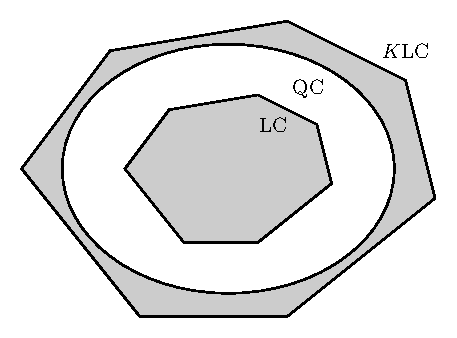
\includegraphics[scale=1]{chapters/fig_QC&LC.pdf}
			\caption{Visualization } \label{fig:QCLC}
		\end{figure}
		
		For the implication of (2) by (1) consider figure \ref{fig:QCLC}. Since $\QC\subset K\LC$ maximizing over the elements in $K\LC$ will result in a better outcome than maximizing over the elements in $\QC$ in the direction of $M$.
		The direction from (1) to (2) we will prove by contraposition. Assume that there is a quantum correlation matrix $A\in\QC_{m,n}$ such that $A\notin K\LC_{m,n}$. By the hyperplane separation theorem we can separate $A$ from $K\LC_{m,n}$ by a linear functional since $\LC_{m,n}$ is convex. That is, we can find a matrix $M\in\mathbb{R}^{m\times n}$ and a real number $c$ such that 
		\begin{equation*}
			\trace{MA^\top} \geq c \text{ and } \trace{M(\xi\eta^\top)^\top}\leq c
		\end{equation*}
		for all $\xi\in\{-1,1\}^m,\eta\in\{-1,1\}^n$.
	\end{proof}
\newpage